% JUMP TO LINE 60, 75
\documentclass[preview, margin=0.6in]{standalone}
\usepackage[letterpaper,portrait,top=0.4in, left=0.6in, right=0.6in, bottom=1in]{geometry}

\usepackage{amsmath, amsfonts, amsthm, amssymb}
\usepackage{graphicx, float}
\usepackage{mathtools}
\usepackage{titlesec}
\usepackage{interval}
\usepackage{hyperref}
\usepackage{siunitx}
\usepackage{titling}
\usepackage{vwcol}
\usepackage{setspace}
\usepackage{empheq}
\usepackage{cancel}
\usepackage{esdiff}
\usepackage{multicol}
\usepackage{mdframed}
\usepackage{esdiff}
\usepackage{tikzsymbols}
\usepackage{multicol}
\usepackage{tikz}
\usepackage{varwidth}
\usepackage{parskip}
\usepackage{pgfplots}
\usepackage{mlmodern}
\pgfplotsset{compat=1.18}
\intervalconfig {
	soft open fences
}

\newcommand{\alignedintertext}[1]{%
  \noalign{%
    \vtop{\hsize=\linewidth#1\par
    \expandafter}%
    \expandafter\prevdepth\the\prevdepth
  }%
}

\newtheorem{lemma}{Lemma}

\newcommand*{\problem}[1]{\section*{Problem #1}}
\newcommand*{\aps}{\section*{AP Corner}}
\newcommand*{\deriv}[1][x]{\ensuremath{\dfrac{\mathrm{d}}{\mathrm{d}#1}}}
\newcommand*{\floor}[1]{\ensuremath{\lfloor #1\rfloor}}
\newcommand*{\lheqzero}{\ensuremath{\underset{\text{L'H}}{\overset{\left[\frac00\right]}{=}}}}
\newcommand*{\lheqinfty}{\ensuremath{\underset{\text{L'H}}{\overset{\left[\frac{\infty}{\infty}\right]}{=}}}}

\DeclareMathOperator{\DNE}{DNE}
\DeclareMathOperator{\sgn}{sgn}

\DeclareMathOperator{\arccsc}{arccsc}
\DeclareMathOperator{\arcsec}{arcsec}
\DeclareMathOperator{\arccot}{arccot}

%opening

\title{\vspace*{-40pt}Classwork Set B}
\author{Jayden Li}
\date{\today}
% \allowdisplaybreaks
\postdisplaypenalty=100000

\begin{document}
\setstretch{1.25}
\fontsize{12pt}{12pt}\selectfont
\setlength{\abovedisplayskip}{\abovedisplayskip/2}
\setlength{\belowdisplayskip}{\belowdisplayskip/2}
\setlength{\parindent}{0pt}
\setlength{\parskip}{2ex plus 0.5ex minus 0.2ex}
\maketitle

\section*{Day 1 Problem 8}
\begin{itemize}
	\item[(a)] $c=a-b$.
	\item[(b)] Let $\theta$ be the angle between vectors $a$ and $b$.
		\begin{align*}
			\lVert a-b \rVert^2&=\lVert a \rVert^2 +\lVert b \rVert^2 -2 \lVert a \rVert \lVert b \rVert \cos\theta \\
			(a-b)\cdot(a-b)&=a\cdot a+b \cdot b-2 \lVert a \rVert \lVert b \rVert \cos\theta \\
			\cancel{a\cdot a}\bcancel{-2}a\cdot b+\cancel{b\cdot b}&=\cancel{a\cdot a}+\cancel{b \cdot b}\bcancel{-2} \lVert a \rVert \lVert b \rVert \cos\theta \\
			\Aboxed{a\cdot b&=\lVert a \rVert \lVert b \rVert \cos\theta}
		\end{align*}
\end{itemize}

\section*{Day 2 Problem 5}

Let $OA,OB,OC\in\mathbb R^n$ be vectors with tails at the origin and heads at the poitns $A,B,C$, respectively. These vectors are collinear (and span a line) if and only if they do not form a linearly independent set. For example, the vector $OC$ cannot be expressed as a linear combination of vectors $OA$ and $OB$; there do not exist scalars $a,b\in\mathbb R$ such that $a(OA)+b(OB)=OC$.

\section*{Day 2 Problem 7}
\begin{center}
	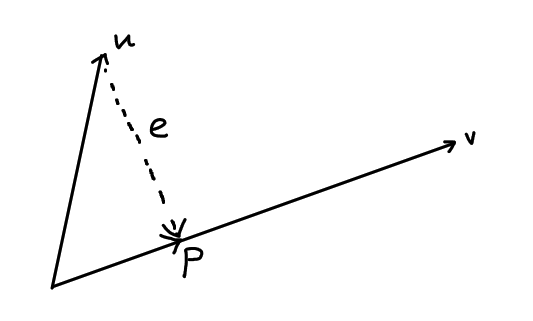
\includegraphics[width=0.6\linewidth]{projection.png}
\end{center}

In the picture above, we have $p=\mathrm{proj}_v(u)$, and vector $e$ is the error between the the projection $p$ and the actual vector $u$: $u+e=p\iff e=p-u$.

The projection $p$ is a scalar multiple of vector $v$. Let $m\in\mathbb R$ be the scalar such that $p=mv$.

Notice that because this is an orthogonal projection, the projection error $e=p-u$ is orthogonal to $v$:
\begin{equation*}
    e\cdot v=0
	\iff (mv-u)\cdot v=0
	\iff m(v\cdot v)=u\cdot v
	\iff m=\frac{u\cdot v}{v\cdot v}
\end{equation*}
With the scalar multiple $m$, we can find the projection $p$:
\begin{equation*}
    \boxed{p 
	=mv
	=\frac{u\cdot v}{v\cdot v}v
	=\frac{u\cdot v}{\lVert v \rVert^2}v}
\end{equation*}

\section*{Day 2 Problem 6}
\begin{equation*}
	\mathrm{proj}_v(u)
	=\frac{u\cdot v}{v\cdot v}v
	=\frac{(3,5)\cdot(6,2)}{(6,2)\cdot(6,2)}(6,2)
	=\frac{18+10}{40}(6,2)
	=\frac{7}{10}(6,2)
	=\boxed{\left( \frac{21}{5},\frac{7}{5} \right)}
\end{equation*}


\end{document}
